\documentclass[UTF8,a4paper,12pt]{ctexart}
\usepackage[a4paper,margin=2.2cm]{geometry}
\usepackage{graphicx,float,booktabs,longtable,xcolor,listings,hyperref}
\hypersetup{colorlinks=true,linkcolor=blue,urlcolor=blue}
\setlength{\parindent}{2em}\setlength{\parskip}{0.45em}\sloppy
\newcommand{\shot}[2]{\begin{figure}[H]\centering\includegraphics[width=0.96\textwidth]{截图/#1}\caption{#2}\end{figure}}
\title{计算机网络技术实践实验四报告\\\large VLAN、Trunk与VLAN间路由}
\author{学号：已隐去}
\date{2026年10月15日}
\begin{document}\maketitle
\begin{abstract}本实验实现三交换机、两路由器和八VLAN的自有拓扑，记录access/trunk、802.1Q标签、跨VLAN路由和两种同LAN多IP方法。当前只完成部分阶段，完整验收仍未通过。\end{abstract}
\section{实验要求与目的}
本实验配置至少三台交换机、两台路由器和八个业务VLAN，验证access、802.1Q trunk、同VLAN跨交换机通信、不同VLAN隔离，以及两种同LAN多IP互联方法。业务VLAN不使用VLAN 1。
\section{拓扑与地址规划}
本设计使用SW1、SW2、SW3，R1、R2和PC20、PC30、PC40、PC50、PC60、PC70、PC80、PC90。地址前缀按学号规则使用205.161；VLAN 20、30、40、50在R1侧，VLAN 60、70、80、90在R2侧，路由器间使用独立互联网段。
\begin{figure}[H]\centering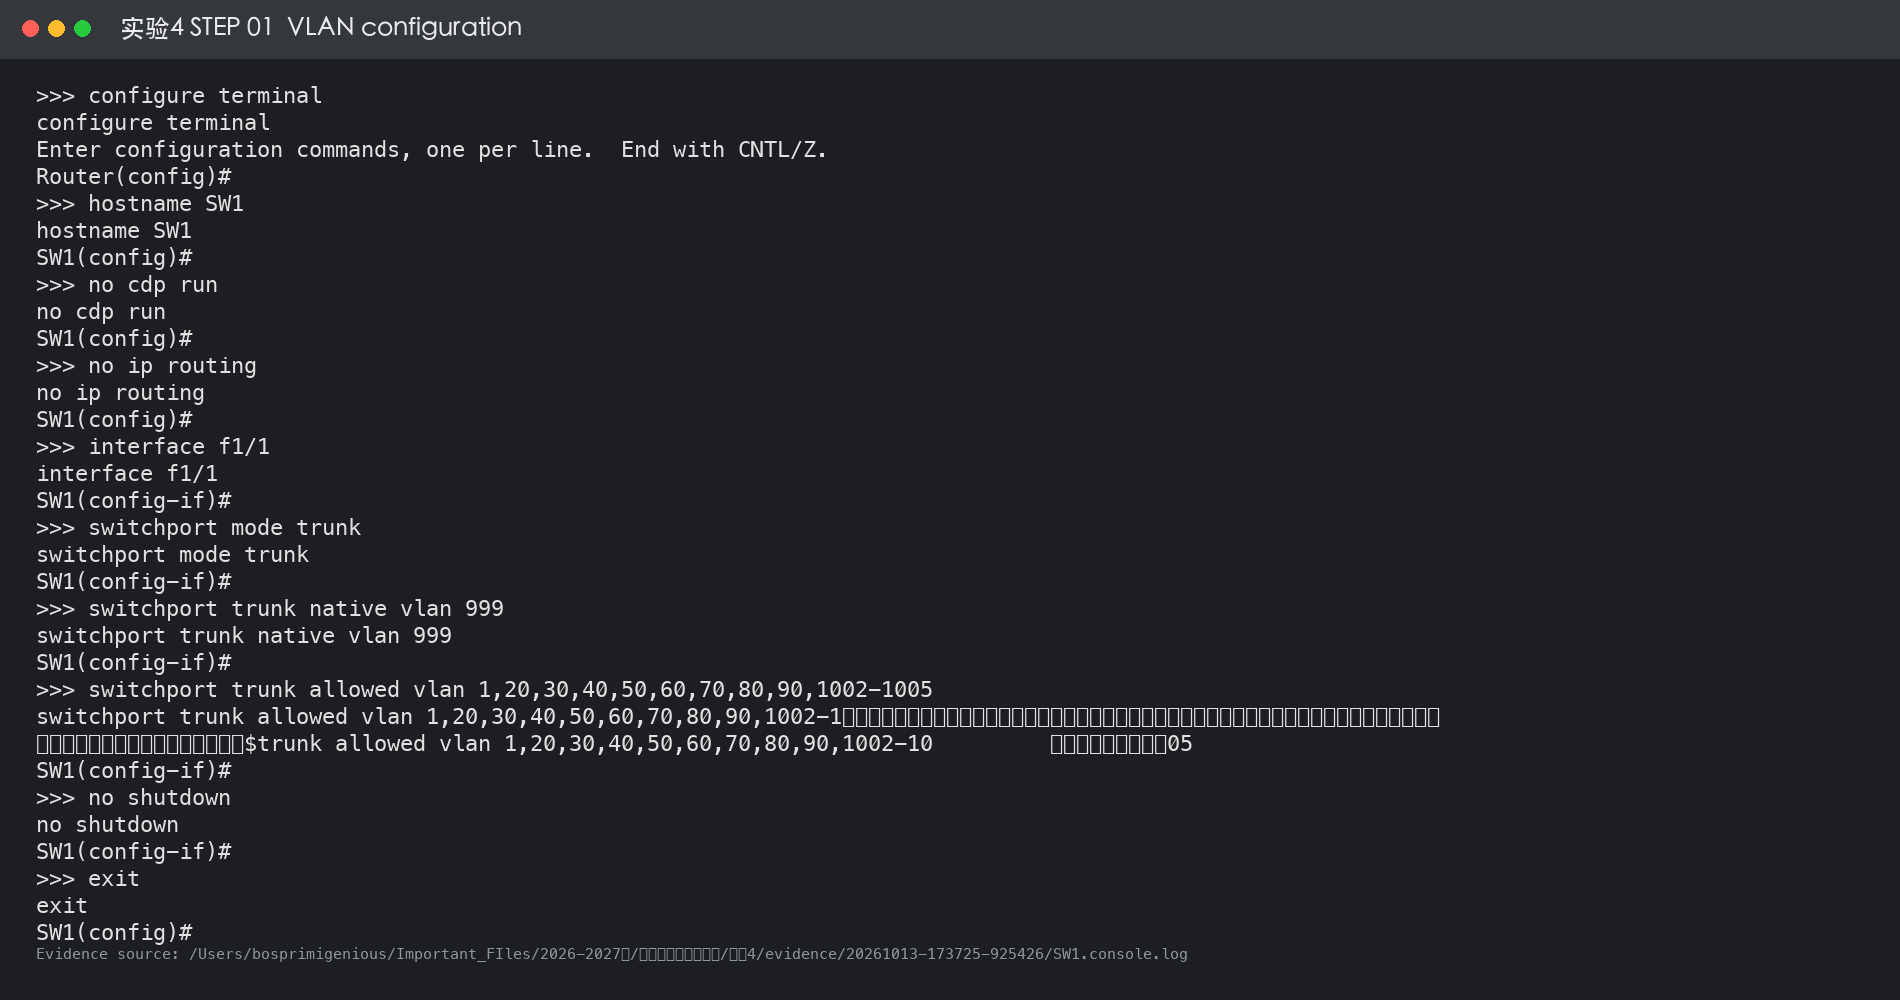
\includegraphics[width=0.96\textwidth]{截图/01-VLAN配置.png}\caption{SW1真实IOS VLAN配置输出。}\end{figure}
\section{VLAN和Trunk配置思路}
先建立业务VLAN并配置access端口，再建立SW1-SW2、SW2-SW3和路由器子接口trunk；trunk允许列表显式包含业务VLAN和IOS默认VLAN，避免NM-16ESW拒绝不完整列表。最后配置R1/R2子接口和物理接口两种互联路径。
\begin{figure}[H]\centering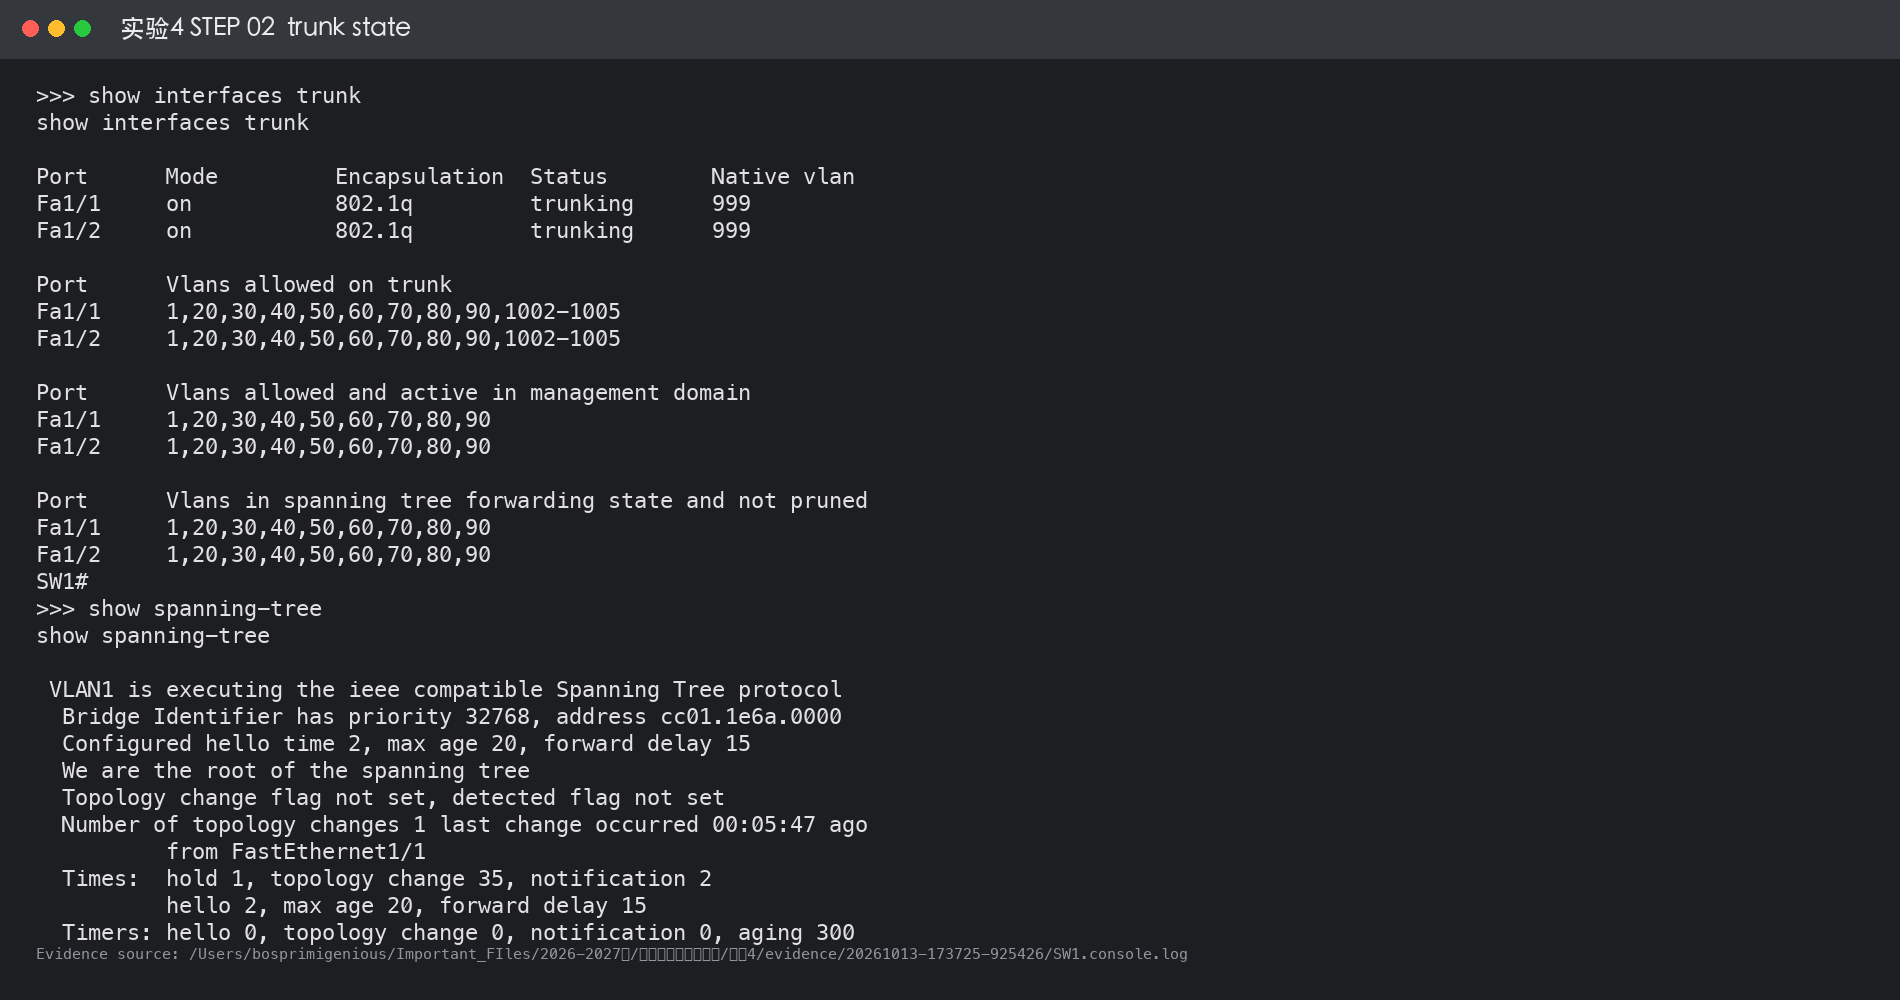
\includegraphics[width=0.96\textwidth]{截图/02-Trunk状态.png}\caption{Trunk状态检查命令与回显。}\end{figure}
\section{分阶段验证}
验收顺序为八VLAN双路由全互通、不同VLAN隔离、同交换机同VLAN、跨交换机同VLAN、同LAN多IP方法一、方法二和恢复配置。每个阶段保留ping和show vlan/trunk/route输出，并采集dot1q、trunk、物理VLAN及路由器互联抓包。
\begin{figure}[H]\centering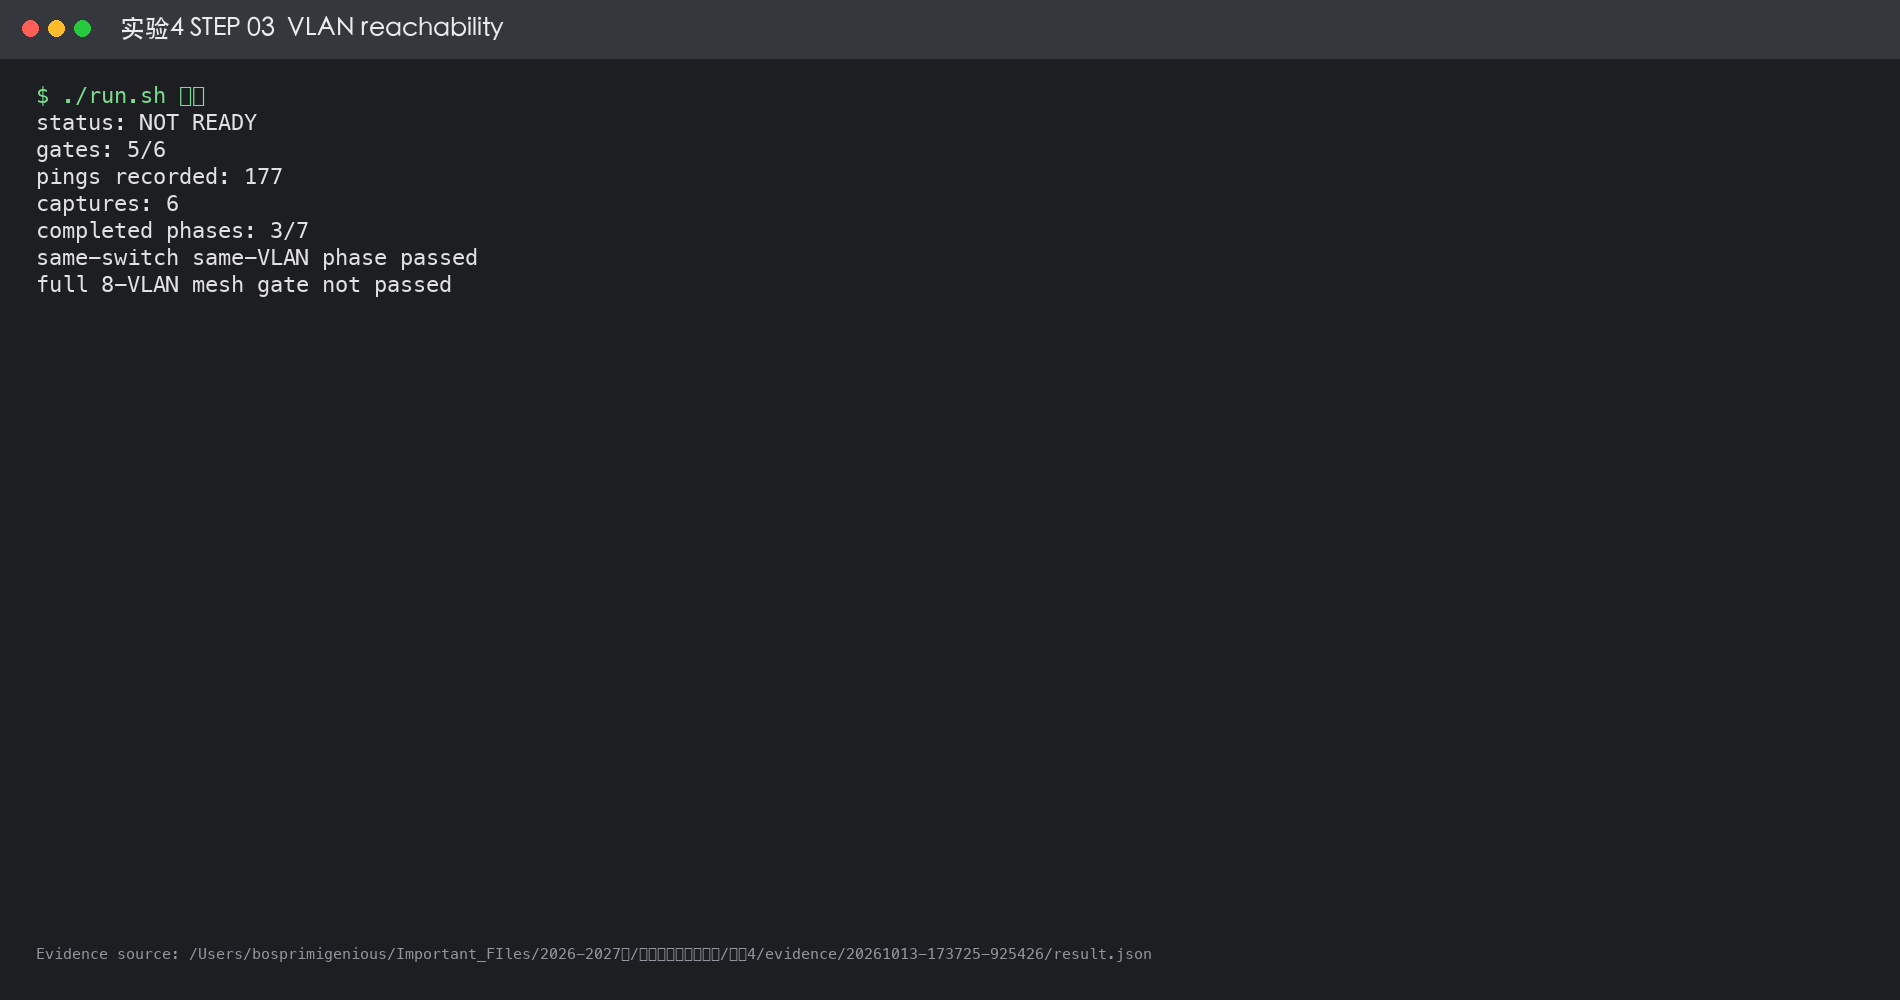
\includegraphics[width=0.96\textwidth]{截图/03-VLAN互ping.png}\caption{已记录阶段和互通门禁摘要。}\end{figure}
\section{当前结果与问题}
当前最完整记录完成3/7阶段，初始部分VLAN互通和隔离阶段有证据，但八VLAN全互通门禁未通过。后续运行遇到DTP异步日志、长命令回显和磁盘写入问题，不能把部分通过写成完整通过；需修正命令回显同步后从空状态重跑七阶段。
\begin{figure}[H]\centering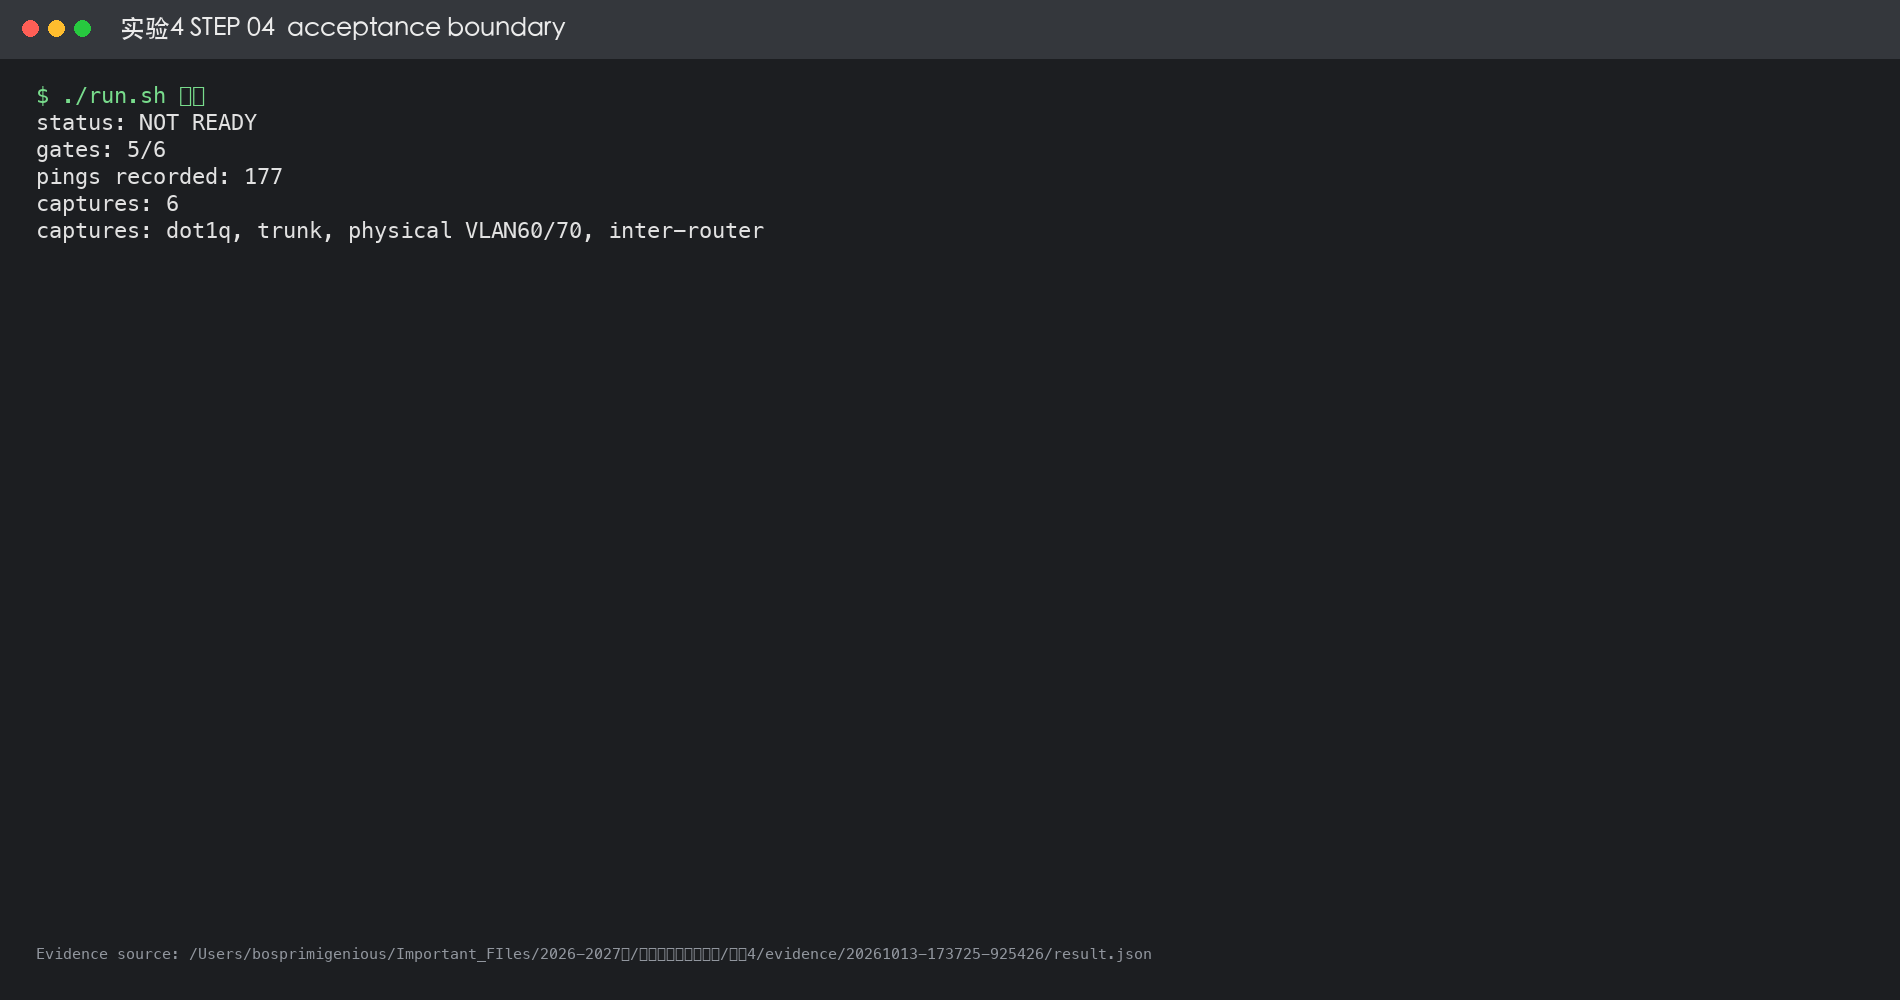
\includegraphics[width=0.96\textwidth]{截图/04-验收状态.png}\caption{实验四当前NOT READY边界。}\end{figure}
\section{截图与证据边界}
本报告的终端图由本项目实际Dynamips/Cisco IOS运行日志和验收JSON生成，原始证据目录保留在本实验的\texttt{evidence/}中。截图展示命令与回显，不把上游报告结果当作本实验结果。当前状态为\textbf{NOT READY}。
\section{结论}
本实验的拓扑、命令和部分阶段已经实现，但存在未通过门禁或外部环境阻塞；本报告记录当前证据，不能将其表述为完整通过。

\end{document}
